\section{Design}
The following chapter is going to cover the design process for the development of the application. By the end of this design chapter it will be clear of the chosen technologies and a high level knowledge of how the system will function will be understood. As part of the design existing map applications such as Google maps \& waze where looked at. Looking at existing map applications allowed the designs to be inspired from different sections and provide and idea of how these systems work, one great side effect of using these systems as inspiration is that it's hoped the system will be clear how to use by user's that have expierence with them.

\subsection{User stories}
User stories are an excellent way of creating more detailed requirements for development. The user stories found within Appendix \ref{appendix:userstories} cover all of the requirements laid out, and also contain a set of user stories each. The implementation of acceptance testing on each user story will provide the basis for testing of the system.

\subsection{Decided technologies}
Programming languages and libraries are very varied and people have many opinions on these. In general a chosen technology, library or language comes down to the developers preference/what they most comfortable in. Several languages have been decided for the final product and the below section is highlighting these along with what influenced the decision.

\subsubsection{Security}
Many people these days like SSO systems allowing them to sign in from their social media accounts. For this reason an SSO provider will be used in order to protect the REST API and web application.

\subsubsection{Rest API}
The rest API is going to be developed using Golang, Golang support module development, is easy to work with and has a performance between Java and C. The author has an interest in this language and wants to reinforce in it and feels this is an excellent use case for this, and will allow expandability of the application in the future.

\subsubsection{Web Application}
The web application will be written within Typescript using the react libary. The main influencing decision for this is the author's interest in keeping up with current popular technologies and feels this would be a good chance to implement the library and develop a progressive web app, and learn about the react libary.

\subsubsection{Android Application}
It has been decided the android application will be written using the traditional Java method as opposed to the current default language of Kotlin, the reason for this is because the author is more familiar with Java and is already using new technologies for the web application. Time limitations mean it's not practical to learn Kotlin in addition to the other technologies for this project rendering it out of scope.

\pagebreak
\subsection{Architecture overview}
With the system being modular and containing several key parts that need to function appropriately together and architecture overview diagram (see figure \ref{fig:architectureov}) has been generated to show how the system intends to work. This architecture overview is useful for understanding the base system that has been implemented.
\begin{figure}[h]
	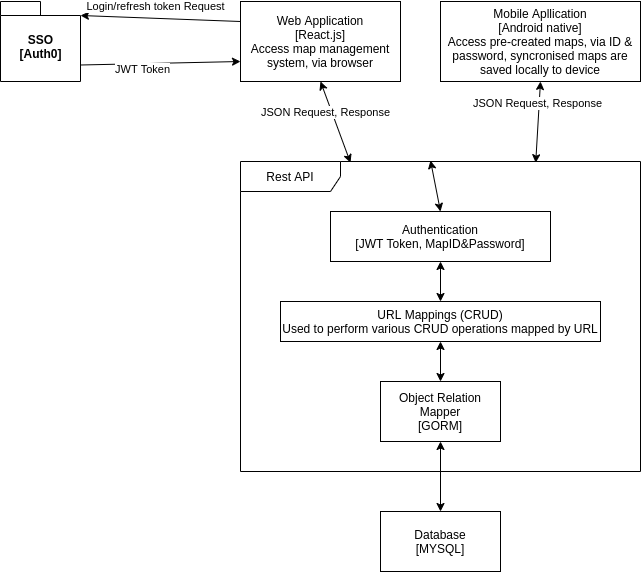
\includegraphics[width=\linewidth]{./images/designs/ArchitectureOverview.png}\\
	\caption{Architecture Overview}
	\label{fig:architectureov}
\end{figure}

\subsection{Data Storage \& Data Structure}
Before development of any new functionality or system it's important to consider the data that's required. The format and quality of the data structure is important the success of a system and is also important to ensure maintainability and expansion is possible in the future. One common storage structure for data is a relational database, this allows quick and easy access and filtering of the data within and is the industry standard. A key method of designing these databases is with an entity relationship diagram (ERD) see figure \ref{fig:erd}.

\begin{figure}[h]
	\centering
	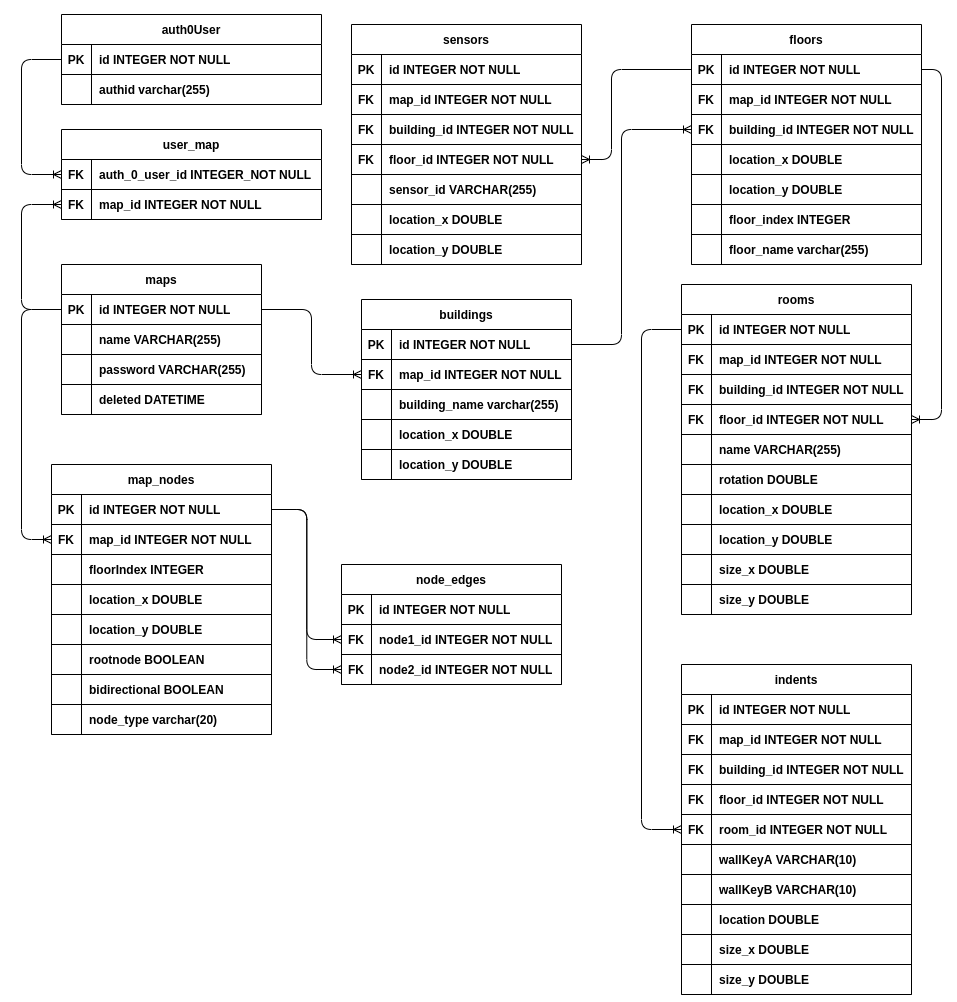
\includegraphics[width=.9\linewidth]{./images/designs/erddetailed.png}\\
	\caption{Entity relationship diagram}
	\label{fig:erd}
\end{figure}

Figure \ref{fig:erd} contains all the key information required to create the initial database for the project, in addition it also gives and insight for all the data needed in the base model for anything that uses this data from the API, as such will serve as a base for creating the Java classes and Golang structs. 

Finally the above diagram also highlights some of the design considerations that where made to make development of the project faster, the first of these was to store rooms as rectangles with overlays as another rectangle, this achieves a more simplistic data structure and types to work with in order to make building the prototype faster. Looking at existing indoor maps of a range of locations such as UWE on google maps, shows that most rooms within a building are rectangular with indents cut out of them, as such a majority of situations will be covered by this data structure,as this is a prototype small limitations are out of scope however if this was to become a business based implementation changes would be required to cover certain edge cases such as the hexagon at UWE, this being said the system will still be capable of demonstrating it's potential within the industry as a prototype.

\subsubsection{Other Data storage}
The rest API will feature the data structure and be connected to a database as above, to allow for quick access and query of data. This isn't needed for the android application and as such the data returned from the rest API will be stored as JSON files on the device. This allows quick serialisation/de-serialisation of data whilst maintaining a simple storage method. This is justified by the fact that the map data will not need to be queried unless already loaded into memory. Using a database would also complicate the re-synchronisation of changed map data.

\newpage
\subsection{REST API Design}
With the data structure defined above, the rest API for this project will perform mostly CRUD operations protected using Auth0, as such no direct design will be done for the rest API, the aim of this section is to give a basic overview of how the rest API will function.

Each data layer will also contain the heirarchial format IE: room update URL would be:\\ /map/buildings/rooms/\{id\}. Each piece of data will contain a route to create, retrieve, update \& delete the piece of data. All routes will be protected via a JWT token which will be supplied by the react application, example URL's and methods for the map itself can be viewed below.

\begin{longtable}{| p{0.2\linewidth} | p{0.1\linewidth} | p{0.7\linewidth}|}
	\hline
	End point & Methods & Description \& Returned data\\\hline
	/maps/\{id\} & GET & Returns whole map data including all child components for the requested ID\\\hline
	/maps/\{id\} & POST & Updates the map only omiting any child elements  returning the new updated map data\\\hline
	/maps/\{id\} & DELETE & Deletes the resource from the service\\\hline
	/maps/ & POST & An empty request will create a blank map, a request containing JSON will be parsed to a full map saving the full map to the database returning new map data\\\hline
	
\end{longtable}

An additional route of just /maps will exist to retrieve top level map data for all maps of the logged in user. This route will have a HTTP method of GET and will take no URL parameters or information, it will however be protected by a JWT token.
Finally one last route will exist ontop of the map which will have the URL of /map/sync which will be used by the android application to syncronise new maps, it will be a post function and will contain formatted json of the mapID and password required, this route will not require any middleware and will be open to use.

\subsection{UI Designs}
There exists a range of map applications already implemented including Google maps, Waze \& apple Maps, with large companies having the budget to design optimum and efficient UI's the designs of the product will be heavily influenced by these applications. Both the android application and web application will have there designs as images, and have an explanation of any functionality/links that are not clear from the designs. All designs have been carefully considered to ensure a complete fulfilment of the requirements.

\pagebreak
\subsubsection{Android Application}
Figure \ref{fig:mapselection} contains the two main states for the map selection screen of the android application, figure \ref{fig:mapselnomap} contains the view if the user has no synchronised map on their device whereas figure \ref{fig:mapselwithmap} contains the view if the user has maps synchronised. It can be noted there is a plus button to synchronise a new map and a filter box to search the synchronised maps for if the user has many, the designed for both of these can be found within figure \ref{fig:mapselectionpopup}.\\
\begin{figure}[h]
	\centering
\begin{subfigure}{.5\textwidth}
	\centering
	\fbox{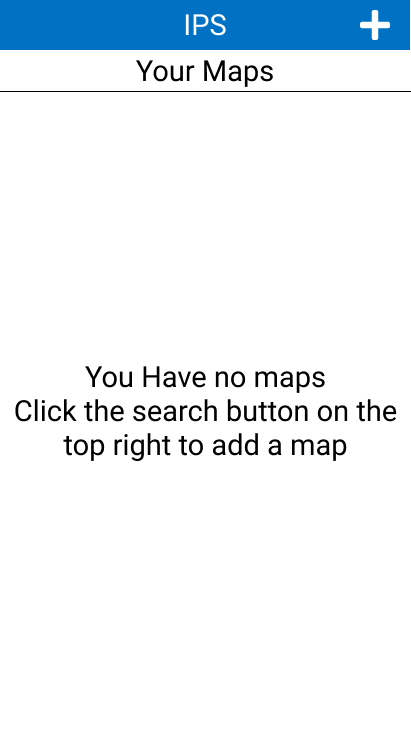
\includegraphics[width=.75\linewidth]{./images/designs/ui/android/MapSelection.png}}
	\caption{Map selection screen when user has no maps}
	\label{fig:mapselnomap}
\end{subfigure}%
\begin{subfigure}{.5\textwidth}
	\centering
	\fbox{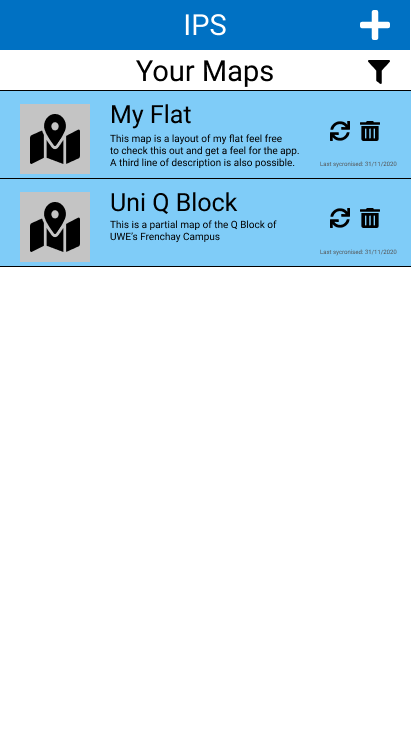
\includegraphics[width=.75\linewidth]{./images/designs/ui/android/MapSelectionWithmaps.png}}
	\caption{Map selection screen when user has maps}
	\label{fig:mapselwithmap}
\end{subfigure}
\caption{Map Selection screen}
\label{fig:mapselection}
\end{figure}
\pagebreak
\begin{figure}[h]
	\centering
	\begin{subfigure}[t]{.5\textwidth}
		\centering
		\fbox{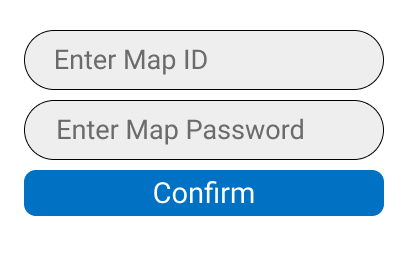
\includegraphics[width=1\linewidth]{./images/designs/ui/android/AddMap.png}}
		\label{fig:mapselpopupsync}
	\end{subfigure}%
	\begin{subfigure}[t]{.5\textwidth}
		\centering
		\fbox{\includegraphics[width=.4\linewidth]{./images/designs/ui/android/mapFilterOveralay.png}}
		\label{fig:mapselpopupfilter}
	\end{subfigure}
	\caption{Map Selection screen popups}
	\label{fig:mapselectionpopup}
\end{figure}

The second key activity for the android app is the positioning activity figure \ref{fig:locationactivity} contains the base view for what this area of the application looks like. It should be noted here there is a hamburger menu overlay see figure \ref{fig:locationpopupsearch}. In addition, to this there is a route options popup the design of which can be seen within \ref{fig:locationpopupoptions}. As with the previous set of designs these cover all the basis for the requirements set out for the application.
\begin{figure}[h]
	\centering
	\fbox{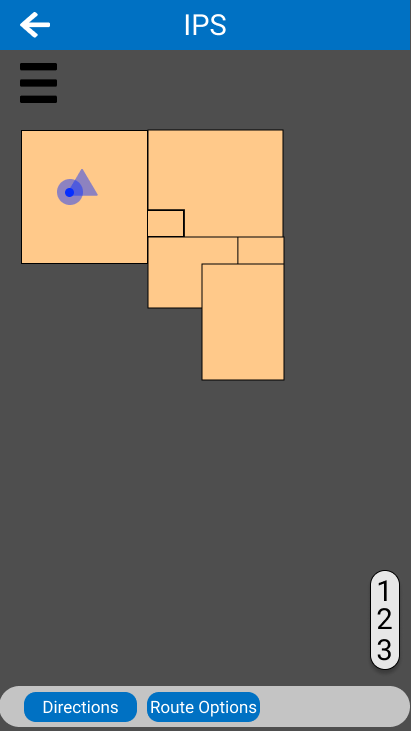
\includegraphics[width={0.3\linewidth}]{./images/designs/ui/android/Map.png}}
	\caption{Main screen of location activity}
	\label{fig:locationactivity}
\end{figure}
Sub Screens\\
\begin{figure}[h]
	\centering
	\begin{subfigure}[h]{.5\textwidth}
		\centering
		\fbox{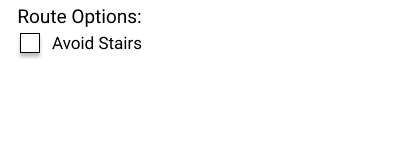
\includegraphics[width=.75\textwidth]{./images/designs/ui/android/RouteOptions.png}}\\
		\caption{}
		\label{fig:locationpopupoptions}
	\end{subfigure}%
	\begin{subfigure}[h]{.5\textwidth}
		\centering
		\fbox{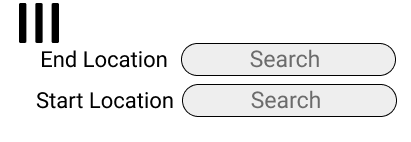
\includegraphics[width=.75\textwidth]{./images/designs/ui/android/RouteSearch.png}}\\
		\caption{}
		\label{fig:locationpopupsearch}
	\end{subfigure}
	\caption{Location popups/overlays}
	\label{fig:locationpopup}
\end{figure}


\pagebreak
\subsubsection{Web Application}
As with the android application the web application has 2 core states, the first is the map selection screen see figure \ref{fig:webappmapsel} which contains the design for this screen. What cannot be seen on this design is when using this page hovering over a map option will present a selection of options including rename and delete located on the top right of the container.\\
\begin{figure}[h]
	\centering
	\fbox{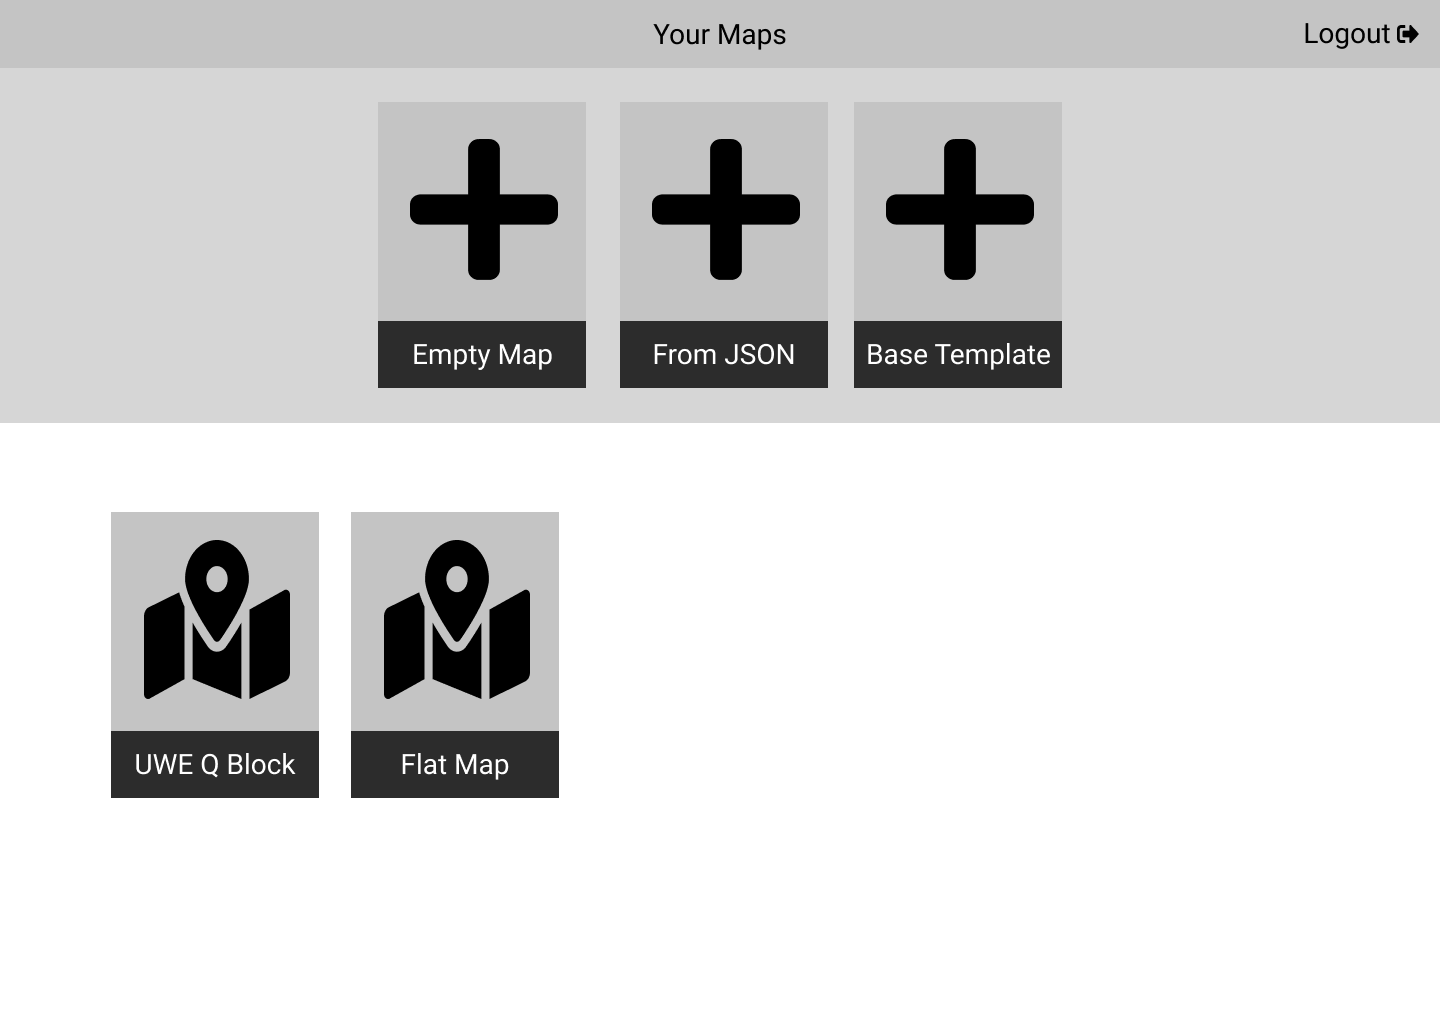
\includegraphics[width=\linewidth]{./images/designs/ui/web/MapSelection.png}}
	\caption{Map selection screen}
	\label{fig:webappmapsel}
\end{figure}

The second state see figure \ref{fig:webappmapeditor} contains the design for the core map editor. Some key elements to note on this design is the tool box on the top left of the canvas which allows interaction with the canvas to do different tasks. The design also features a hierarchy based component, this component is a list selection for the levels of the data structure allowing addition, editing and deleting of the element at each level. Finally there is a QR generation button which will generate a QR code to scan by an android device to synchronise the map to the device.
\begin{figure}[h]
	\centering
	\fbox{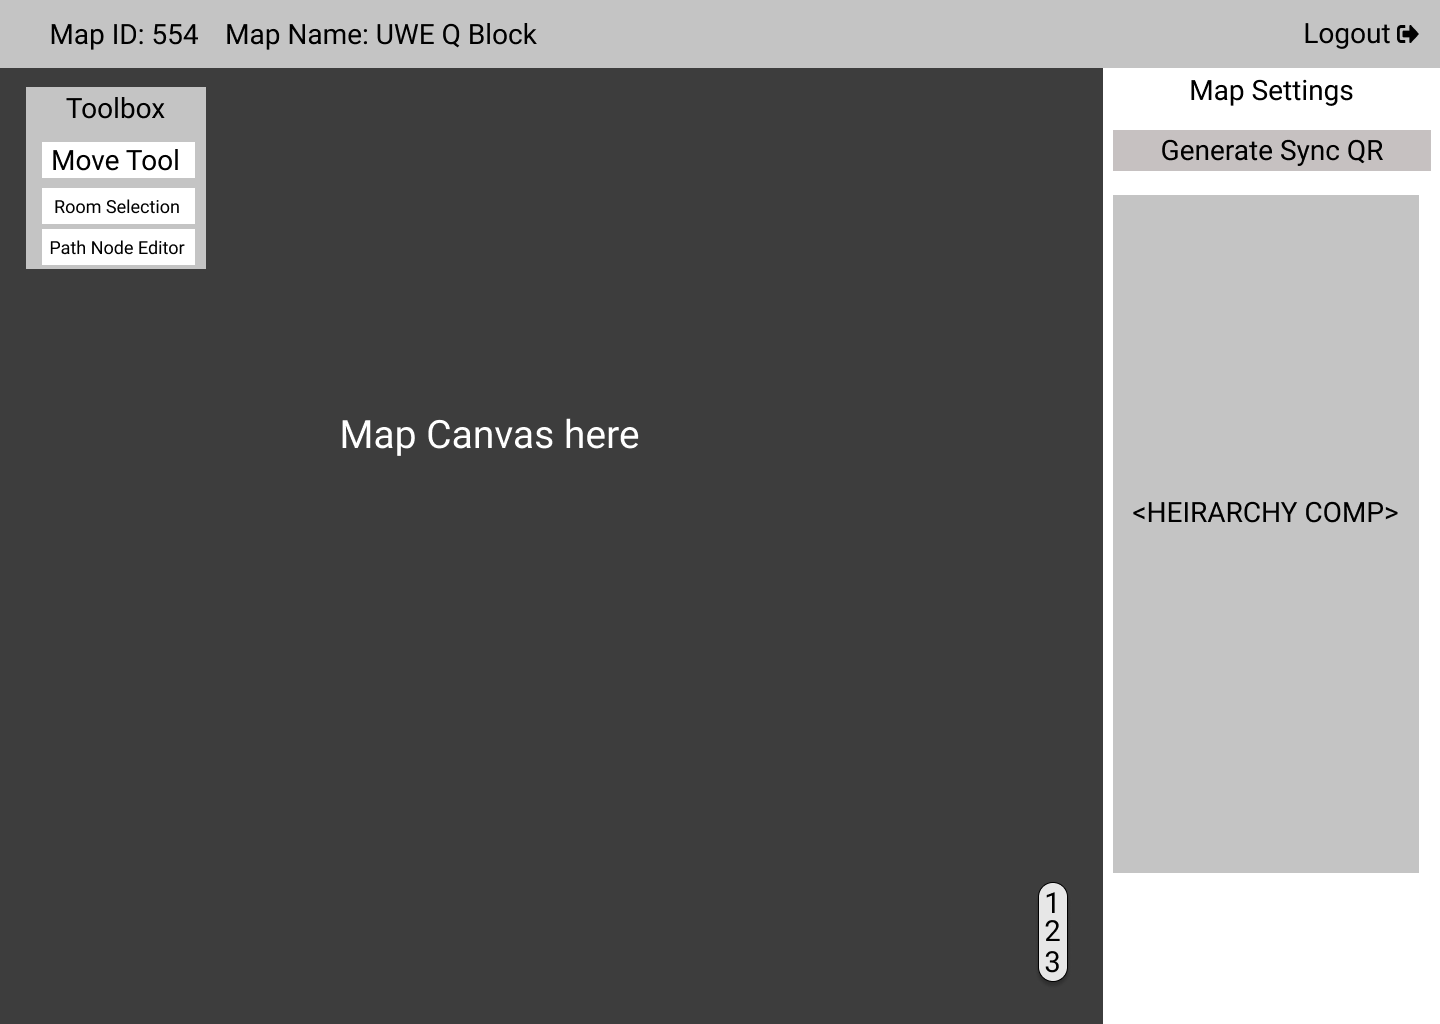
\includegraphics[width=\linewidth]{./images/designs/ui/web/MapEditor.png}}
	\caption{Map selection screen}
	\label{fig:webappmapeditor}
\end{figure}

Finally designs for the Dashboard as defined in requirement \ref{web:dashboard} have been omitted due to having a priority of could. The designs for this element will be visited if there is time in the future to complete this requirement
\pagebreak
\subsection{Important design considerations}
As with any system making it generic and expandable is something to consider from an early stage. Not doing this can be detrimental to the long term standing of the code making it more difficult to expand and improve the application with time.

One key area for expandability was found within the research where by UWB appear's to be the future of indoor positioning systems due it traction building from addition of smart phones, IOT and other devices. As such, Bluetooth is the optimal solution for the projects aims and objectives currently although that will probably change in the future. For this reason it's important to consider the integration of Bluetooth and potentially other sensor's into the positioning calculation. For this reason several interfaces will exist on the implementation, the lowest interface will contain a list of scan and distance services, passing all sensor ID's to them so results can be filtered. The idea of the scan and distance service is to return a set of formatted data back from it's implementation, this means any sensor can be used, and calculation of distance can be changed per sensor type. One the location service has ran these functions for all the different sensors the system can then use this data to calculate the location as identified within the research.

Another important design approach is to keep the code as independent from the system as possible, doing so will allow the ability to create a library that is used in the future. It also means that the system is easier to maintain and can be ported to other systems that run the JDK with minimal work. Finally it's important to ensure a clear distinction between the view and logic, implementing a new UI shouldn't interfere with any core system logic, methods exist for this already as such a Model View Controller approach will be used for the whole system this again ensures expandability and ease of development in the future.